\chapter{\ifproject%
\ifcpe การทดลองและผลลัพธ์\else Experimentation and Results\fi
\else%
\ifcpe การประเมินระบบ\else System Evaluation\fi
\fi}

\CIreply{อธิบายภาพรวมโดยคร่าวๆ ให้เห็นส่วนประกอบของบทนี้ ก่อนเข้าสู่แต่ละหัวข้อ}

\section{Feedback จากทาง nursery}
(รูปที่~\ref{fig:Feedback})
\CIreply{ไม่ต้องใส่รูป เขียนสรุปให้ครบประเด็น}
สรุปเป็นหัวข้อหลักๆได้ดังต่อนี้
\paragraph{ระบบบัญชี}
\begin{itemize}
    \item ยังไม่มีใบแจ้งยอดและใบเสร็จ
    \item ใบเสร็จไม่สามารถแนบสลิปจากภายนอกได้
    \item การเพิ่มรายการบัญชีไม่สามารถเลือกประเภทของสิ่งของต่างๆได้ 
\end{itemize}
\paragraph{ระบบคลังสินค้า}
\begin{itemize}
    \item ราคาของสินค้าไม่สามารถแก้ไขได้
    \item ไม่สามารถหักจำนวนของสินค้าอัตโนมัติได้
\end{itemize}
\CIreply{unclear อันนี้ feedback ตอนไหน เขียนให้ชัด ไม่เห็น timeline เลย}

\section{แก้ไขตาม feedback}
\CIreply{ใช้เวลาแก้ไขนานเท่าไร}
\paragraph{ระบบบัญชี}
\begin{itemize}
    \item ออกแบบให้ใช้งานได้ง่ายมากยิ่งขึ้น (รูปที่~\ref{fig:Payment})
    \item เพิ่มใบเสร็จและใบแจ้งยอด (รูปที่~\ref{fig:slipPage}, \ref{fig:invoicePage})
    \item ใบเสร็จสามารถแนบสลิปจากภายนอกได้ (รูปที่~\ref{fig:updatePayment})
    \item การเพิ่มรายการบัญชีสามารถเลือกประเภทของสิ่งของต่างๆได้ (รูปที่~\ref{fig:CreatePayment})
\end{itemize}
\paragraph{ระบบคลังสินค้า}
\begin{itemize}
    \item ออกแบบให้ใช้งานได้ง่ายมากยิ่งขึ้น (รูปที่~\ref{fig:Stock})
    \item ราคาของสินค้าสามารถแก้ไขได้ (รูปที่~\ref{fig:editPrice})
    \item สามารถหักจำนวนของสินค้าอัตโนมัติได้ (รูปที่~\ref{fig:CheckStock}, \ref{fig:HistoryStock})
\end{itemize}
\paragraph{หน้าประวัติ}
\begin{itemize}
    \item แก้ไขให้ใช้งานง่ายมากยิ่งขึ้น (รูปที่~\ref{fig:Profile})
\end{itemize}

\CIreply{ลงรายละเอียดว่าของเก่ามันไม่ดีอย่างไร และเราแก้ไขอย่างไรให้มันดีขึ้น}

\section{ผลลัพธ์จากการประเมินหลังจากมีการแก้ไขตาม feedback}
\CIreply{เขียนบรรยายสรุปผลการประเมินด้วย อย่าให้คนอ่านมองแต่รูปภาพ}
(รูปที่~\ref{fig:Eval1}, \ref{fig:Eval2}, \ref{fig:Eval3}, \ref{fig:Eval4}, \ref{fig:Eval5}, \ref{fig:Eval6}, \ref{fig:Eval7}, \ref{fig:Eval8})

\begin{figure}
  \begin{center}
    
\includegraphics[width=\linewidth]{images/feedback.png}
  \end{center}
  \caption[หน้า feedback จากทาง nursery]{Feedbackจากทางnursery}
  \label{fig:Feedback}
\end{figure}
\begin{figure}
  \begin{center}
    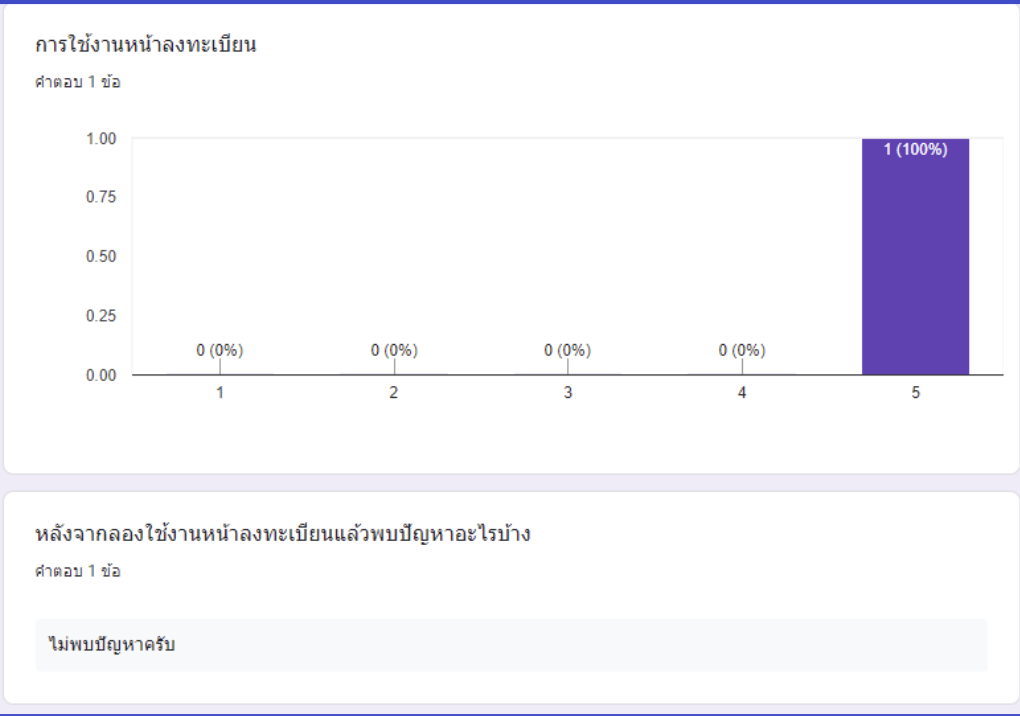
\includegraphics[width=\linewidth]{images/eval1.png}
  \end{center}
  \caption[ผลลัพธ์จากการประเมินการใช้งาน หน้าลงทะเบียน]{ผลลัพธ์จากการประเมินการใช้งาน หน้าลงทะเบียน}
  \label{fig:Eval1}
\end{figure}

\begin{figure}
  \begin{center}
    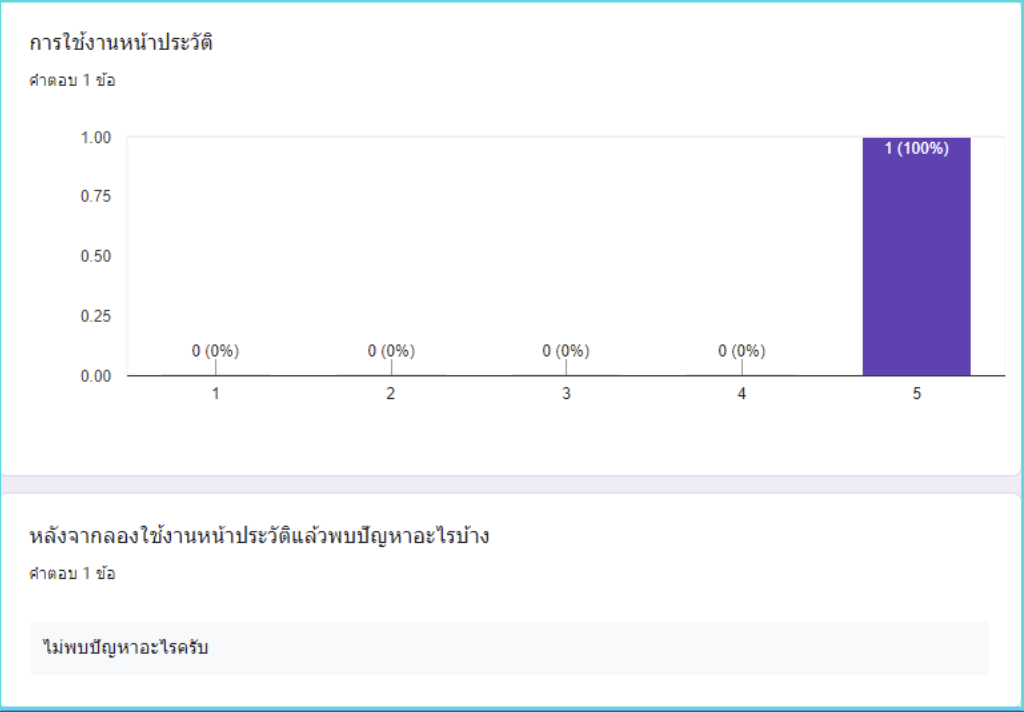
\includegraphics[width=\linewidth]{images/eval2.png}
  \end{center}
  \caption[ผลลัพธ์จากการประเมินการใช้งาน หน้าประวัติ]{ผลลัพธ์จากการประเมินการใช้งาน หน้าประวัติ}
  \label{fig:Eval2}
\end{figure}

\begin{figure}
  \begin{center}
    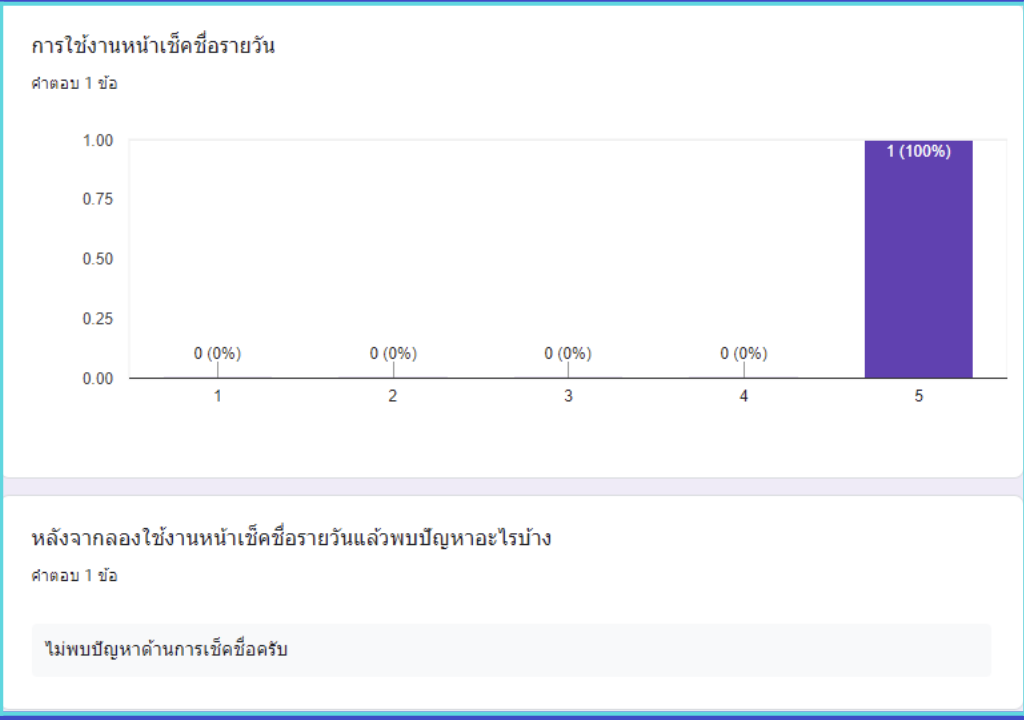
\includegraphics[width=\linewidth]{images/eval3.png}
  \end{center}
  \caption[ผลลัพธ์จากการประเมินการใช้งาน หน้าประวัติ]{ผลลัพธ์จากการประเมินการใช้งาน หน้าเช็คข้อมูลรายวัน}
  \label{fig:Eval3}
\end{figure}

\begin{figure}
  \begin{center}
    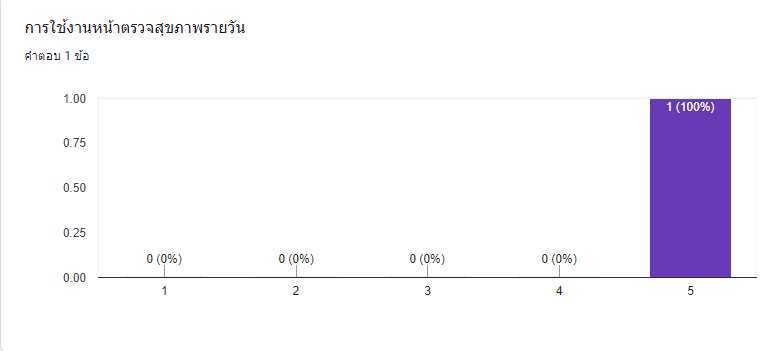
\includegraphics[width=\linewidth]{images/eval5.png}
  \end{center}
  \caption[ผลลัพธ์จากการประเมินการใช้งาน ตรวจสุขภาพรายวัน]{ผลลัพธ์จากการประเมินการใช้งาน ตรวจสุขภาพรายวัน}
  \label{fig:Eval5}
\end{figure}

\begin{figure}
  \begin{center}
    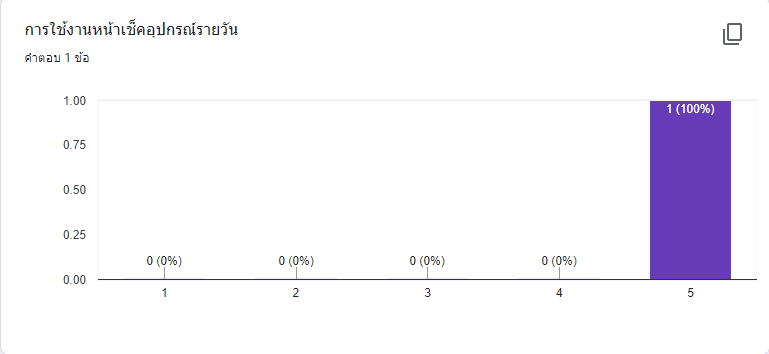
\includegraphics[width=\linewidth]{images/eval6.png}
  \end{center}
  \caption[ผลลัพธ์จากการประเมินการใช้งาน เช็คอุปกรณ์รายวัน]{ผลลัพธ์จากการประเมินการใช้งาน เช็คอุปกรณ์รายวัน}
  \label{fig:Eval6}
\end{figure}

\begin{figure}
  \begin{center}
    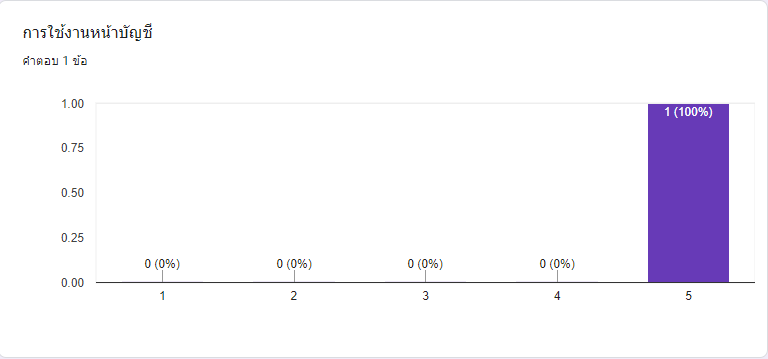
\includegraphics[width=\linewidth]{images/eval7.png}
  \end{center}
  \caption[ผลลัพธ์จากการประเมินการใช้งาน ระบบบัญชี]{ผลลัพธ์จากการประเมินการใช้งาน ระบบบัญชี}
  \label{fig:Eval7}
\end{figure}

\begin{figure}
  \begin{center}
    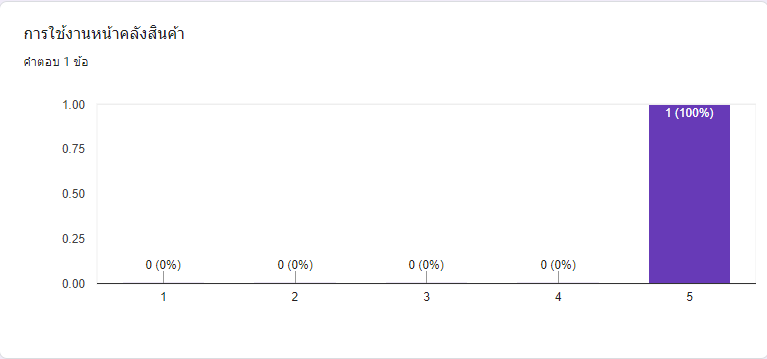
\includegraphics[width=\linewidth]{images/eval8.png}
  \end{center}
  \caption[ผลลัพธ์จากการประเมินการใช้งาน ระบบคลังสินค้า]{ผลลัพธ์จากการประเมินการใช้งาน ระบบคลังสินค้า}
  \label{fig:Eval8}
\end{figure}

\begin{figure}
  \begin{center}
    
\includegraphics[width=\linewidth]{images/eval4.png}
  \end{center}
  \caption[Comment จากผู้ใช้งาน]{Comment จากผู้ใช้งาน}
  \label{fig:Eval4}
\end{figure}





